\chapter{Results and Discussion}
\section{Flow Visualization}
The simulation is done with $xstart = 250$, $xend = 482.7$ and the spatial oscillation occurs at wavelength of $\lambda = 58$. The graphical representation are shown by figure~\ref{fig:w(f(x))} and~\ref{fig:w(x,z)}. 
\begin{figure}[h]
  \centering
  \scalebox{0.7}{\includegraphics{figures/w(f(x))_t7000.pdf}}
  \caption{Two dimensional contour plots of wall oscillation at $y=0:w(f(x))|_{y=0}$ with \emph{xstart} = 250, \emph{xend} = 482.7 and $\lambda$ = 58}
  \label{fig:w(f(x))}
\end{figure}

\begin{figure}[h]
  \centering
  %\scalebox{0.7}{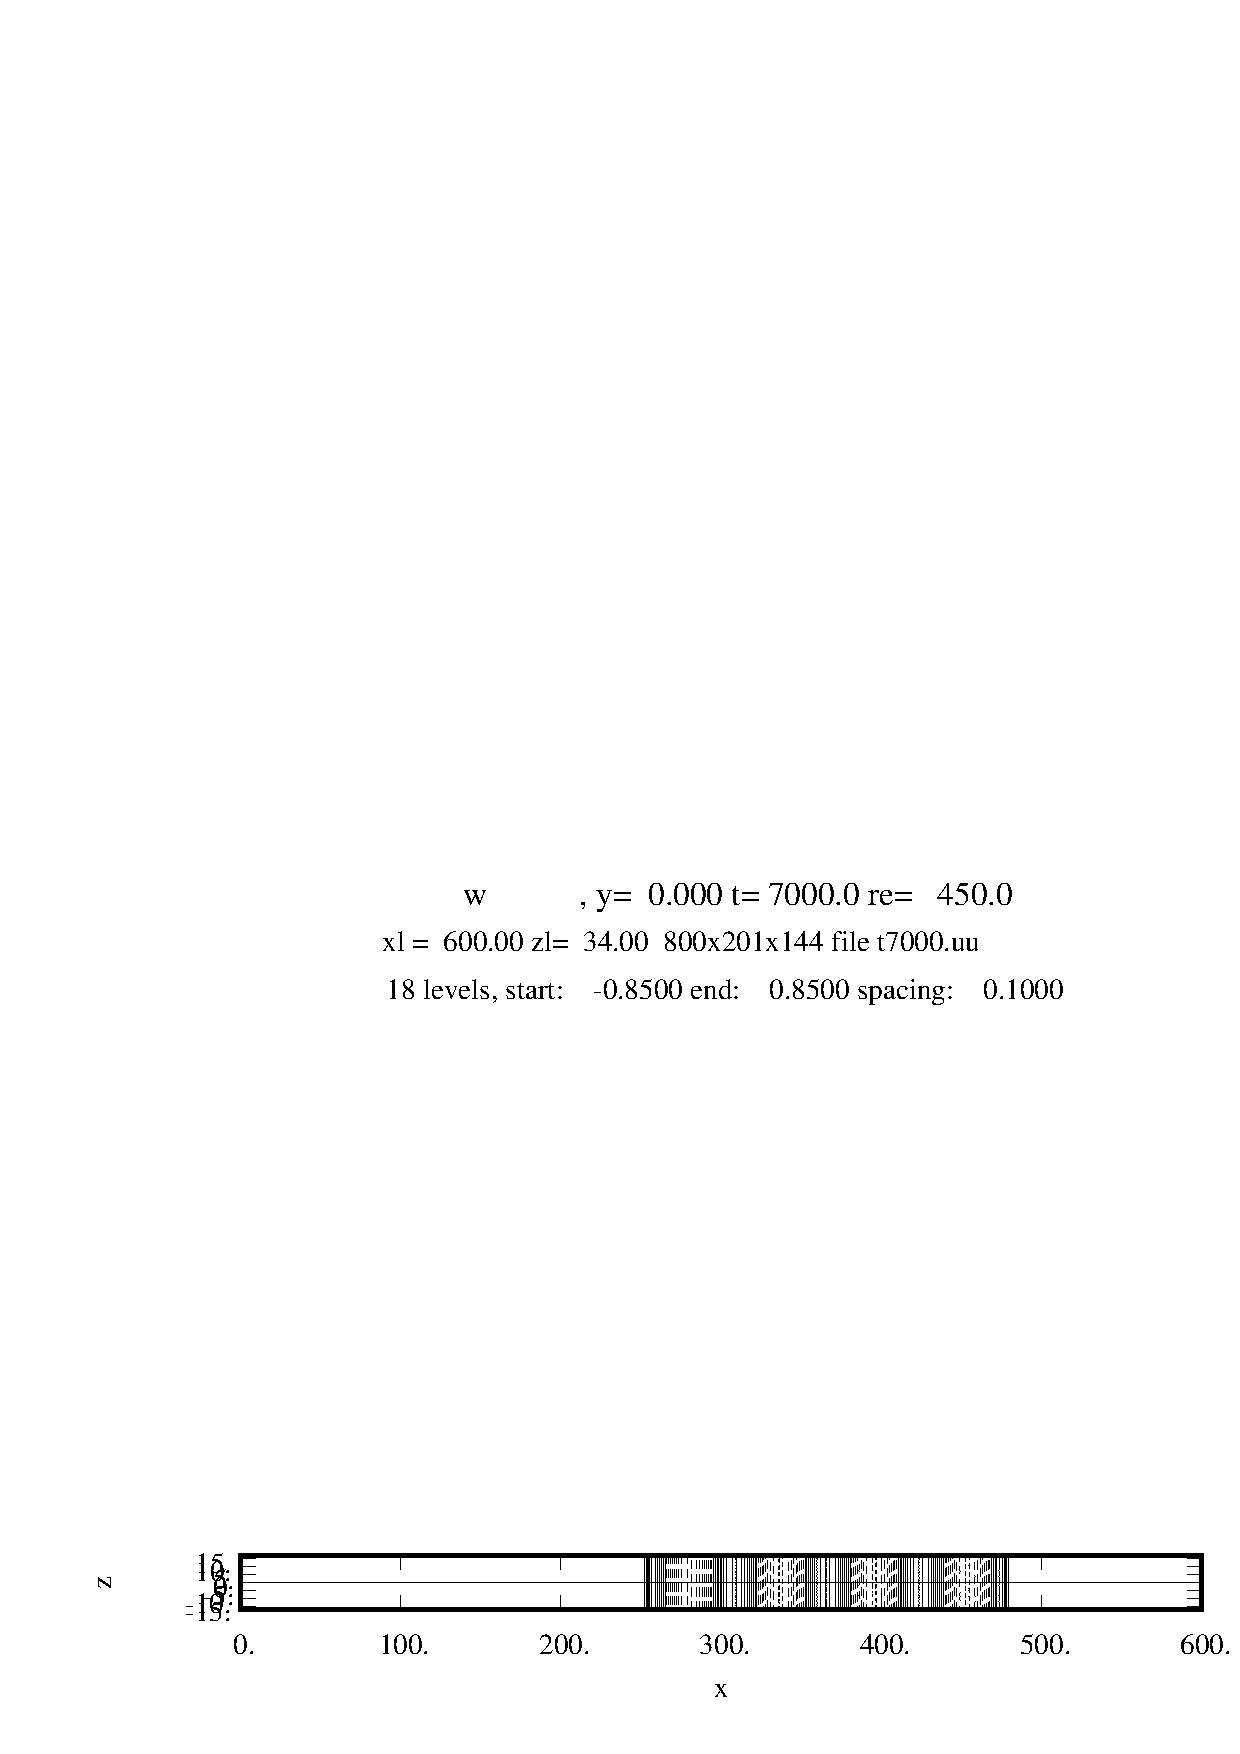
\includegraphics{figures/w(x,z).pdf}}
  \includegraphics[width=15cm]{figures/w_4.pdf}
  \caption{Two dimensional contour plots of wall oscillation at $y=0:w(x,z)|_{y=0}$ with \emph{xstart} = 250, \emph{xend} = 482.7 and $\lambda$ = 58}
  \label{fig:w(x,z)}
\end{figure}

\subsection{Streamwise Velocity Field}
Streamwise velocity field refers to the \emph{x}-component of the velocity vector of the fluid. It has the direction parallel to the plate along the fluid stream. In standard notation, it is represented by variable \emph{u}. In this project, only two-dimensional contour plots will be given.

Since there are great ratio difference between x and y-direction, an equal ratio plot will not produce good flow visual. To improve the visibility, y-direction is stretched to accommodate the length of x-direction.

In this simulation, the wall oscillation is started from $xstart = 250$ to $xend = 487.2$. In accordance with the step function, the inflow and outflow of the computational box is laminar flow. This is followed by the transition area, which is shown by the slope on the function. The flow image is plotted by using 20 contour. Two dimensional contour plot of streamwise velocity field in plane $z=0$ at $t = 19600$ can be seen in figure~\ref{fig:u(x,y)}.

\begin{figure}[!h]
  \centering
  \scalebox{0.7}{\includegraphics{figures/u(x,y)_t19600.pdf}}
  \caption{Streamwise velocity field at $t = 19600$ }
  \label{fig:u(x,y)}
\end{figure}

In the area where the wall oscillation is applied, it can be seen that the velocity field are looser than its counterpart. However, in the near wall region, the velocity field has no significant change.

\subsection{Wall Normal Velocity Field}
Wall normal velocity field refers to the \emph{y}-component of the velocity vector of the fluid. It has direction perpendicular to the plate. In standard notation, it is represented by variable \emph{v}.

Since there are great ratio difference between x and y-direction, an equal ratio plot will not produce good flow visual. To improve the visibility, y-direction is stretched to accommodate the length of x-direction.

In this simulation, the wall oscillation is started from $xstart = 250$ to $xend = 487.2$. The flow image is plotted by using 20 contour. Two dimensional contour plot of wall normal velocity field in plane $z=0$ at $t = 19600$ can be seen in figure~\ref{fig:v(x,y)}.

\begin{figure}[!h]
  \centering
  \scalebox{0.7}{\includegraphics{figures/v(x,y)_t19600.pdf}}
  \caption{Wall normal velocity field at $t = 19600$}
  \label{fig:v(x,y)}
\end{figure}

The introduction of wall oscillation in wall normal direction will thin away at the near wall region. This is shown by the difference of space between left and right part of computational box, in which more space can be found at $x=250-500$ region.

\subsection{Spanwise Velocity Field}
Wall normal velocity field refers to the \emph{z}-component of the velocity vector of the fluid. It has directions parallel to the plate and parallel to the width dimension of the plate. In standard notation, it is represented by variable \emph{w}.

Since there are great ratio difference between x and y-direction, an equal ratio plot will not produce good flow visual. To improve the visibility, y-direction is stretched to accommodate the length of x-direction.

In this simulation, the wall oscillation is started from $xstart = 250$ to $xend = 487.2$. The flow image is plotted by using 20 contour. Two dimensional contour plot of spanwise velocity field in plane $z=0$ at $t = 19600$ can  be seen in figure~\ref{fig:w(x,y)}.

\begin{figure}[!h]
  \centering
  \scalebox{0.7}{\includegraphics{figures/w(x,y)_t19600.pdf}}
  \caption{Spanwise velocity field at $t = 19600$}
  \label{fig:w(x,y)}
\end{figure}

In spanwise velocity field it can be seen the application of wall oscillation will cause the velocity field to thicken in the near wall region. This is shown by the flow lines which stack together at $x=250-500$ compared to the flow lines at $x=0-250$ where more space can be found in the near wall region.

\subsection{Streamwise Velocity Fluctuations}
The fluctuation of streamwise velocity field is obtained by applying gaussian anisotropic high-pass filter to the streamwise velocity field. This filter removes the mean value of the streamwise velocity, hence displaying the low-speed and high-speed streak of the streamwise velocity.

Figure~\ref{fig:svl_0-250} shows the streamwise velocity fluctuations at $x = 0 - 250$. It can be seen that when the flow is not exposed to oscillation, the box is full of fluctuation. This is in contrast with the condition shown in figure~\ref{fig:svl_250-500}. At position $x = 250 -500$, when the flow is exposed to oscillation, the box is has less fluctuation compared to the previous position. With decreasing number of fluctuations it can be assumed that the drag at that location is reduced. This assumption will be further discussed in the next section.  

\begin{figure}[!h]
  \centering
  \subfloat[$x=0 - 250$]{\label{fig:svl_0-250}\scalebox{0.7}{\includegraphics{figures/w(x,z)_0-250.pdf}}} \\
  \subfloat[$x=250 - 500$]{\label{fig:osc_0-250}\scalebox{1.05}{\includegraphics{figures/w_x_0-250.pdf}}}
  \caption{Two dimensional contour plots of streamwise velocity field fluctuations at plane $y=1$ at $t= 19600$: -- $u=-0.05$; - - $u=0.05$}
  \label{fig:stream_vel_fluct_0-250}
\end{figure}

\begin{figure}[!h]
  \centering
  \subfloat[$x=0 - 250$]{\label{fig:svl_250-500}\scalebox{0.7}{\includegraphics{figures/w(x,z)_250-500.pdf}}} \\
  \subfloat[$x=250 - 500$]{\label{fig:0sc_250-500}\scalebox{1.05}{\includegraphics{figures/w_x_250-500.pdf}}}
  \caption{Two dimensional contour plots of streamwise velocity field fluctuations at plane $y=1$ at $t= 19600$: -- $u=-0.05$; - - $u=0.05$}
  \label{fig:stream_vel_fluct_250-500}
\end{figure}

\section{Drag reduction}
The investigation of the effect of wall oscillation on drag reduction can be done through skin friction coefficient. The mathematical formulation for skin friction coefficient is shown by equation~\ref{eq:skin_friction}. 
\begin{equation}\label{eq:skin_friction}
  C_f = 2\left(\frac{u_\tau}{U_\infty}\right)
\end{equation}
The friction velocity ($u_\tau$) can be calculated from the mean streamwise velocity gradient at the wall, which is shown in equation~\ref{eq:u_tau}
\begin{equation}\label{eq:u_tau}
  u_\tau = \sqrt{v\left.\frac{\partial u}{\partial y}\right|_{y=0}}
\end{equation} 

Figure~\ref{fig:cf_all} shows the skin friction coefficient $(C_f)$ as function of streawise coordinate $(x)$. To avoid the confusion caused by the numerical effects, the graph is shown in the range of $x=150$ to $x=500$. In figure~\ref{fig:cf_all}, the skin friction coefficient of undisturbed (---) is compared with the simulation results after 200, 400, 600, 800 ($\cdots$) and the total cycles (\textbf{---}).  

\begin{figure}[!h]
  \centering
  \scalebox{1.1}{\includegraphics{figures/cf-total-all.pdf}}
  \caption{Skin friction coefficient (undisturbed (---), 200, 400, 600 and 800 cycles ($\cdots$), total cycles (\textbf{---})). It can be seen that the application of wall oscillation will reduce the skin friction coefficient significantly. The skin friction coefficient is reduced gradually with the increase of time.}
  \label{fig:cf_all}
\end{figure}

Figure~\ref{fig:cf_all} shows that the skin coefficient friction shows reduction at $x=250$ where the oscillation start. At the end of wall oscillation $(x=482.7)$, the skin friction coefficient will gradually return to its original position. The number of cycles also give significant effects to the drag reduction. It can be seen that the drag reduction given by 200 cycles is less than the 600, etc. With the increasing number of cycles, the reduction will eventually reach its constant value which is shown by the results from total cycles (---). 

To see the difference between the effect of spanwise wall oscillation with space variation and time variation, simulation results from previous final year project (---) is compared with current simulation results ($\cdots$). Figure~\ref{fig:cf_compare} shows the comparison of skin friction coefficient between the undisturbed case, time variation and space variation simulations results. Similar to figure~\ref{fig:cf_all}, the simulation box is limited in the range of $x=150$ to $x=500$ to avoid the effect caused by the numerical scheme.

\begin{figure}[!h]
  \centering
  \scalebox{1.1}{\includegraphics{figures/cf-total-compare.pdf}}
  \caption{Skin friction coefficient comparison(temporal (\Cutline), spatial (---)). The spatial variation produce more skin friction coefficient reduction than temporal variation. Note that a pattern similar to wall oscillation exist in spatial variation curve.}
  \label{fig:cf_compare}
\end{figure}

From figure~\ref{fig:cf_compare}, it can be seen that the spanwise wall oscillation with space variation result more drag redu ction compared to time variation (previous case). An interesting behaviour is also shown by the spatial variation simulation results. In the region where the wall oscillation is applied, there is certain pattern that resembles the wall oscillation. This pattern is not found in the simulation results from previous final year project (wall oscillation with time variation). The cause of this pattern is assumed as the effect of the wall oscillation with spatial variation. This assumption is supported by the occurrence with same pattern in other simulation results (200, 400, 600 and 800 cycles) shown in figure~\ref{fig:cf_all}. 

It can be seen that the pattern will gradually form a fixed pattern with the increasing cycles, which is shown by figure~\ref{fig:cf_zoom}. The simulation result with 200 cycles shows a strong pattern, which gradually decrease with the increase of cycles.

\begin{figure}[!h]
  \centering
  \scalebox{1.1}{\includegraphics{figures/cf_zoom.pdf}}
  \caption{Magnified skin friction coefficient (total cycles (\textbf{---}), 200, 400, 600 and 800 cycles ($\cdots$)). The pattern in skin friction coefficient will form a fixed pattern with the increase of time.}
  \label{fig:cf_zoom}
\end{figure}

Percentage of drag reduction can be calculated by using equation~\ref{eq:dr}.
\begin{equation}\label{eq:dr}
  DR(\%) = 100\frac{C_f^0 - C_f}{C_f^0}
\end{equation}
where $C_f^0$ is the reference skin friction coefficient (undisturbed case). 

The maximum percentage of drag reduction for the current project is $46.33\%$ which is $6.33\%$ higher than the drag reduction from previous project. This finding confirmed the result obtained by Viotti and Quadrio~\cite{viotti} that the wall oscillation with spatial variation will produce more drag reduction compared to temporal variation. However, the comparison shows  smaller difference than stated by Viotti and Quadrio which are $20-30\%$. The comparison of percentage of drag reduction for both projects is shown in figure~\ref{fig:dr}. 

\begin{figure}[!h]
  \centering
  \scalebox{1.1}{\includegraphics{figures/dr-total-indras.pdf}}
  \caption{Percentage of drag reduction. Temporal (\Cutline), spatial (---)}
  \label{fig:dr}
\end{figure}

\section{Flow Statistics}
The investigation of the effect of spanwise wall oscillation on the mean flow can be done through the observation of flow statistics.

\begin{figure}[!h]
  \centering
  \subfloat[Velocity profile]{\label{fig:u-y}\scalebox{1.1}{\includegraphics{figures/u_y.pdf}}}\\
  \subfloat[Mean velocity profile]{\label{fig:u_logy}\scalebox{1.1}{\includegraphics{figures/u_logy.pdf}}}
  \caption{(a) Velocity profile at $x=400$, (b) Mean velocity profile with wall scaling. The solid line ($\cdots$) shows the linear profile $(u+=y+)$}
\end{figure}

The velocity profile of the flow at $x=400$ is shown in figure~\ref{fig:u-y}. It shows that the spanwise wall oscillation modify the velocity profile. The most significant change on the velocity profile can be seen in its velocity gradient $(\frac{\partial u}{\partial y})$. The reference velocity profile (undisturbed case) shows thicker profile compared to the one by spanwise wall oscillation. From the comparison above, it could be concluded that the velocity gradient of flow with spanwise wall oscillation is smaller than the reference flow, which lead to drag reduction. 

 Comparison between the velocity profile of spanwise wall oscillation with spatial and temporal variation is also shown in figure~\ref{fig:u-y}. The comparison shows that the velocity profile of temporal variation is thicker than the one of spatial variation, which mean the larger velocity gradient.

Figure~\ref{fig:u_logy} shows the mean velocity profile with wall scaling. The velocity profile scaled with $u_{\tau}$ is seen close to the linear profile. When the same velocity profile is scaled with $u_{\tau_0}$ (non-oscillating wall), the profile shift closer to the velocity profile with undisturbed case.

\begin{figure}[!h]
  \centering
  \scalebox{1.1}{\includegraphics{figures/stats_total.pdf}}
  \caption{Total turbulent intensity at $x=400$, the higher value profiles are the reference flow and the lower value profiles are the flow with spatial variation}
  \label{fig:stats_total}
\end{figure}

Another turbulent characteristics affected by spanwise wall oscillation are the turbulent intensities. The comparison between spatial variation scaled with $u_{\tau}$ and undisturbed case turbulent intensities ($u_{rms}+, v_{rms}+ \mbox{ and } -uv+$) is shown in figure~\ref{fig:stats_total}. The reference flow is shown by higher profiles and flow with spatial variation by the lower profiles.

\begin{figure}[!h]
  \centering
  \subfloat[$u_{rms}+$]{\label{fig:urms}\scalebox{1.1}{\includegraphics{figures/urms.pdf}}}\\
  \subfloat[$v_{rms}+$]{\label{fig:vrms}\scalebox{1.1}{\includegraphics{figures/vrms.pdf}}}
  \caption{Turbulent intensity at $x=400$,(a) $u_{rms}+$, (b) $v_{rms}+$, (c) $-uv+$}
  \label{fig:turbulent_intensity}
\end{figure}

\begin{figure}[!h]
  \ContinuedFloat
  \centering
  \subfloat[$-uv+$]{\label{fig:uv}\scalebox{1.1}{\includegraphics{figures/uv.pdf}}}
  \caption{Turbulent intensity at $x=400$,(a) $u_{rms}+$, (b) $v_{rms}+$, (c) $-uv+$}
\end{figure}

For clarity, figure~\ref{fig:turbulent_intensity} shows the turbulent intensities in individual plot. It can be seen the turbulent intensities are reduced when flow is subjected to spanwise wall oscillation. The reduction are $44\%$, $27\%$ and $53\%$ for $u_{rms}+, v_{rms}+ \mbox{ and } -uv+$ respectively. $-uv+$ reduction is notably the largest from all turbulent intensities. Figure~\ref{fig:turbulent_intensity} also shows the comparison between turbulent intensities of flow with spatial and temporal variation. The spanwise wall oscillation with spatial variation cause more reduction of turbulent insensities compared to temporal variation. The reduction for temporal variation are $33\%$, $22\%$ and $40\%$ for $u_{rms}+, v_{rms}+ \mbox{ and } -uv+$ respectively.

\begin{figure}[!h]
  \centering
  \scalebox{0.7}{\includegraphics{figures/vrms+_xy.pdf}}
  \caption{$v_{rms}+$ in $x-y$ field}
  \label{fig:vrms+_xy}
\end{figure}

Figure~\ref{fig:vrms+_xy} shows $v_{rms}$ in $x-y$ field. At $x=0-250$, the profile shows gradual increase of slope (upper part of profile). Wall oscillation is applied at $x=250-500$, this is marked by the oscillation pattern in the lower part of the profile. The introduction of wall oscillation also change the upper part of the profile which is shown by a sudden drop of the profile in \emph{y}-direction.

\begin{figure}[!h]
  \centering
  \scalebox{0.7}{\includegraphics{figures/w_x.pdf}}
  \caption{Side by side Comparison between mean velocity profile in lateral direction with Stoke's second problem.}
  \label{fig:stokes}
\end{figure}

Comparison between mean velocity profile in the lateral direction and Stoke's second problem is shown in figure~\ref{fig:stokes}. It can be seen that both cases have the similar profile.

Further observation on turbulent properties on lateral direction shows some unexpected results. The turbulent intensities for lateral direction shows unusual behaviour when compared to turbulent intensities in other direction. Turbulent intensities for lateral direction are shown in figure~\ref{fig:wrms+_xy}.

\begin{figure}[!h]
  \centering
  \scalebox{0.7}{\includegraphics{figures/wrms+_xy.pdf}}
  \caption{$w_{rms}+$ in $x-y$ field}
  \label{fig:wrms+_xy}
\end{figure}

Figure~\ref{fig:wrms+_xy} shows $w_{rms}$ in $x-y$ field. On the left side of the computational box ($x=0-250$), the flow lines are very close to surface. It change when the wall oscillation is introduced at $x=250-500$. In this position, the space between the flow lines and surface is widening.

The comparison of $w_{rms}$ at various $x$ position can be seen in figure~\ref{fig:wrms_comparison}. An interesting pattern can be observed at turbulent intensities in lateral direction, where the variation of turbulent intensities can be seen when the oscillation is at maximum or minimum value and at zero value. The cause of this irregularities is not known. It is recommended to do further investigation at this phenomena. 

\begin{figure}[h]
  \centering
  \scalebox{1.1}{\includegraphics{figures/wrms-all.pdf}}
  \caption{Comparison of $w_{rms}$ on various positions}
  \label{fig:wrms_comparison}
\end{figure}
